\section{Wikipedia assignment: EE 102 in the wild}
This year in EE 102, we are exploring a new way to learn concepts related to signal processing by connecting it to the real world. We will do this by editing Wikipedia articles related to EE 102. This Wikipedia assignment will help you connect EE 102 with applications, people, instruments, and
ideas beyond our lectures. You have been assigned a team at random on CatCourses. Each team will learn about a signal processing
topic, research published sources, and contribute a clear, well-supported
writeup (with sources) to its Wikipedia article. You are writing for readers outside this
class and helping them understand something you have learned.

\textbf{Grading}: The Wikipedia assignment is part of Midterm \#3. The Wikipedia assignment contributes
\textbf{20 points}, and the written exam contributes \textbf{80 points}.

\subsection{First step: Register on the course dashboard}
Last week's announcement introduced the assignment. If you have not
registered yet, please get started now:
\begin{enumerate}
    \item Find your team in
    \href{https://catcourses.ucmerced.edu/courses/39201/groups\#tab-9972}{the CatCourses group list}.
    \item Create or sign in to your own Wikipedia account and
    \href{https://dashboard.wikiedu.org/courses/UC_Merced/Signal_Processing_and_Linear_Systems_(Fall_2026)?enroll=kzbshpao}{enroll in our Wiki Education course dashboard}.
    Each team member should enroll.
    \item Start the
    \href{https://dashboard.wikiedu.org/training/students/wikipedia-essentials}{Wikipedia policies training module}
    linked in the announcement. Then follow the assigned training and
    activities on our dashboard.
\end{enumerate}

The activities of this week on the Wiki Education dashboard that are due this week are shown in the image below:
\begin{figure}[t]
    \centering
    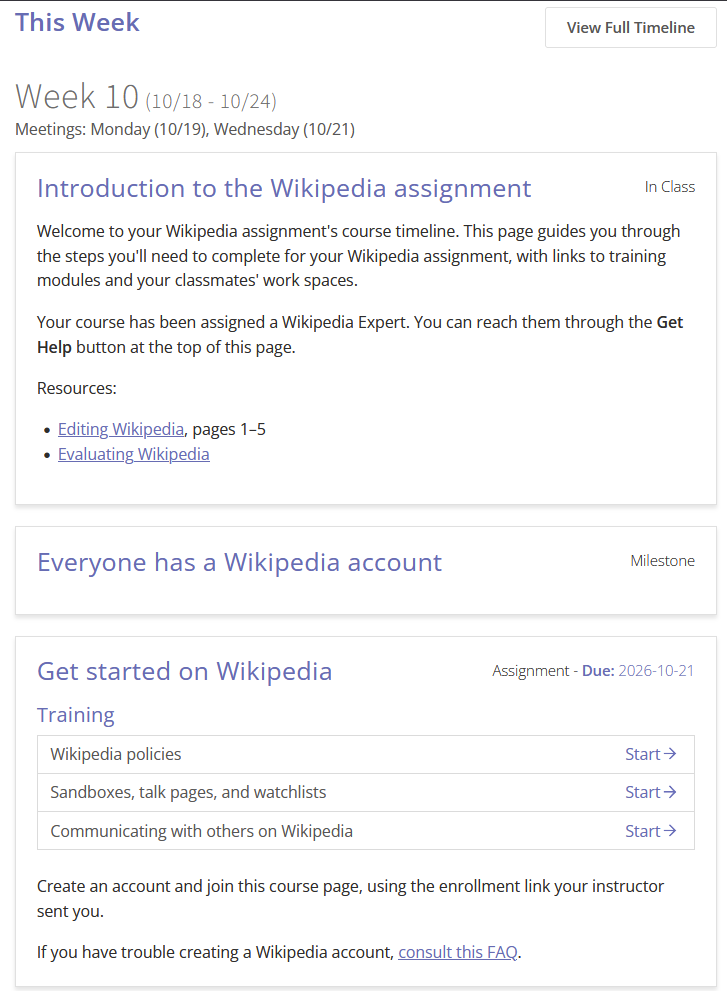
\includegraphics[width=0.5\textwidth]{wikipedia_assignment_week10_tasks.png}
    \caption{The Wiki Education dashboard shows the activities assigned to our course.}
    \label{fig:dashboard}
\end{figure}



\subsection{Possible topics for EE 102}
You can explore topics we have not yet studied in detail. Look for a clear
connection to signals, systems, frequency content, or the history of these
ideas. Some possible directions could be:
\begin{itemize}
    \item \textbf{Audio and music:} pitch, timbre, noise reduction, or the
    \href{https://en.wikipedia.org/wiki/Phase_vocoder}{phase vocoder}.
    Research how time- and frequency-domain descriptions support a specific
    audio technique or application.
    \item \textbf{Scientific instruments:} lock-in amplifier,
    oscilloscopes, or spectrum analyzers. Explore how an instrument extracts
    useful information from a measured signal.
    \item \textbf{Signals in other fields:} EEG/ECG recordings, seismic
    signals, or sonar. A focused application can connect our mathematical
    tools to measurements and questions in another discipline.
    \item \textbf{History and people:} the development of harmonic analysis,
    early sound-analysis instruments, or a documented contribution to
    signal-processing history. Research the context and evidence behind
    the development, as well as the technical idea.
\end{itemize}

\section{Midterm course feedback}
Please fill out the survey called \textbf{Midterm course feedback} when it
is launched on CatCourses. Use it to share what is helping you learn and
what could improve the second half of the course.
